\documentclass[a4paper]{article}
\usepackage[a4paper,margin=0mm]{geometry}
\usepackage{fontspec}
\usepackage{unicode-math}
\usepackage{tikz}
\usetikzlibrary{fit,calc,positioning,arrows.meta}
\usepackage[table]{xcolor}
\usepackage[absolute]{textpos}
\usepackage{array}

\setmainfont{Libertinus Serif}
\setsansfont{Libertinus Sans}
\setmathfont{Libertinus Math}

\definecolor{accent}{HTML}{0F6A52}
\definecolor{badge}{HTML}{A9CFC2}
\definecolor{ink}{HTML}{2A2E30}

\setlength{\TPHorizModule}{1mm}
\setlength{\TPVertModule}{1mm}
\setlength{\parindent}{0pt}
\pagestyle{empty}

\newcommand{\topicheader}[2]{%
\begin{textblock*}{194mm}(16mm,10mm)
\begin{tikzpicture}
\node[fill=accent,text=white,font=\sffamily\bfseries\fontsize{13}{13}\selectfont,
      minimum width=9mm,minimum height=9mm,inner sep=0pt] at (4.5mm,-4.5mm) {#1};
\node[font=\sffamily\bfseries\fontsize{15}{16}\selectfont,text=ink,anchor=west] at (12mm,-4.5mm) {#2};
\end{tikzpicture}
\end{textblock*}
\begin{textblock*}{194mm}(16mm,22.5mm)

\begin{tikzpicture}
\fill[accent] (0,0) rectangle (194mm,0.5mm);
\end{tikzpicture}
\end{textblock*}
}

\newcommand{\pagekicker}[1]{%
\begin{textblock*}{100mm}(16mm,25.5mm)
\begin{tikzpicture}
\node[fill=ink,text=white,font=\sffamily\bfseries\fontsize{8}{8}\selectfont,
      inner sep=2.2pt,rounded corners=1pt] {\MakeUppercase{#1}};
\end{tikzpicture}
\end{textblock*}
}

\newcommand{\videobanner}[1]{%
\begin{textblock*}{178mm}(16mm,25.5mm)
\begin{tikzpicture}
\fill[accent] (0,0) rectangle (178mm,-10mm);
\draw[white,line width=0.6pt] (3mm,-1.7mm) rectangle (11.5mm,-8.3mm);
\node[white,font=\sffamily\fontsize{4}{4.4}\selectfont,align=center] at (7.25mm,-5mm) {QR\\CODE};
\node[white,font=\sffamily\bfseries\fontsize{9.5}{11}\selectfont,anchor=west] at (16mm,-5.6mm) {WATCH THE VIDEO BEFORE YOU SOLVE};
\node[white,font=\sffamily\fontsize{7.5}{8}\selectfont,anchor=east] at (174mm,-5.6mm) {YouTube ~\textbullet~ #1};
\end{tikzpicture}
\end{textblock*}
}

\newcommand{\pagefooter}[1]{%
\begin{textblock*}{194mm}(8mm,286.41mm)
  
\begin{tikzpicture}
    \fill[accent] (0,0) rectangle (194mm,0.6mm);
  \end{tikzpicture}
\end{textblock*}
\begin{textblock*}{63.59mm}(8mm,288.27mm)
  {\sffamily\bfseries\color{accent}\fontsize{13}{16}\selectfont SAT 1200+}
\end{textblock*}
\begin{textblock*}{10mm}(188mm,288.27mm)
  \centering{\sffamily\color{accent}\fontsize{14}{16}\selectfont #1}
\end{textblock*}
}

\newcommand{\cardbg}[4]{%
\begin{textblock*}{#3mm}(#1mm,#2mm)
\begin{tikzpicture}
\fill[badge!22,rounded corners=3mm] (0,0) rectangle (#3mm,-#4mm);
\end{tikzpicture}
\end{textblock*}%
}

\newcommand{\pill}[3]{%
\begin{textblock*}{160mm}(#1mm,#2mm)
\begin{tikzpicture}
\node[fill=accent,text=white,anchor=north west,font=\sffamily\bfseries\fontsize{10}{10}\selectfont,
      rounded corners=8pt,inner xsep=5mm,inner ysep=1.8mm] at (0,0) {RULE ~\textperiodcentered~ #3};
\end{tikzpicture}
\end{textblock*}%
}

\newcommand{\pillw}[3]{%
\begin{textblock*}{160mm}(#1mm,#2mm)
\begin{tikzpicture}
\node[fill=accent,text=white,anchor=north west,font=\sffamily\bfseries\fontsize{10}{10}\selectfont,
      rounded corners=8pt,inner xsep=5mm,inner ysep=1.8mm] at (0,0) {#3};
\end{tikzpicture}
\end{textblock*}%
}

\arrayrulecolor{accent}
\setlength{\arrayrulewidth}{0.7pt}
\renewcommand{\arraystretch}{1.5}


% Bar graph (histogram of counts). #1 counts, #2 slot width mm, #3 mm per count,
% #4 number of bars, #5 total picture height mm, #6 mean (x position), #7 top of mean line (count units)
\newcommand{\bargraph}[7]{%
\pgfmathsetmacro{\bgW}{#4*#2}%
\pgfmathsetmacro{\bgS}{#5-5}%
\begin{tikzpicture}[x=#2mm,y=#3mm]
\useasboundingbox (0mm,-#5mm) rectangle (\bgW mm,0mm);
\begin{scope}[shift={(0mm,-\bgS mm)}]
\draw[ink!55,line width=0.5pt] (0.3,0) -- ({#4+0.7},0);
\foreach \c [count=\i] in {#1} {%
  \ifnum\c>0 \fill[accent] ({\i-0.42},0) rectangle ({\i+0.42},\c);\fi
  \node[below,font=\sffamily\fontsize{6}{6}\selectfont,text=ink!80,inner sep=1pt] at (\i,0) {\i};
}
\draw[dashed,ink!70,line width=0.45pt] (#6,-0.2) -- (#6,#7);
\node[above,font=\sffamily\fontsize{5.5}{6}\selectfont,text=ink!80,inner sep=1pt] at (#6,#7) {mean};
\end{scope}
\end{tikzpicture}}

\begin{document}
\topicheader{7}{Data Analysis Edge Cases}
\videobanner{Lesson 7}
\pagefooter{97}
\mbox{}%
% ---- Mean, median, mode (y=40.0 h=46.3 end 86.3)
\cardbg{16}{40.0}{178}{46.3}
\pill{26}{43.0}{Mean, median, mode}
\begin{textblock*}{158mm}(26mm,52.5mm)
{\fontsize{15}{18}\selectfont mean $=\dfrac{\text{total}}{\text{count}}$ \quad median $=$ middle value \quad mode $=$ most frequent}
\end{textblock*}
\begin{textblock*}{158mm}(26mm,65.2mm)
{\fontsize{13}{16}\selectfont even count: median $=$ average of the two middle values}
\end{textblock*}
\begin{textblock*}{158mm}(26mm,71.7mm)
{\fontsize{13}{16}\selectfont mean of 5 is $30$, mean of the other 4 is $28$: \ removed $=5(30)-4(28)=38$}
\end{textblock*}
\begin{textblock*}{158mm}(26mm,78.1mm)
{\itshape\color{black!70}\fontsize{11}{14}\selectfont Work with totals, not means.}
\end{textblock*}
% ---- Add, remove or change a value (y=91.8 h=38.9 end 130.7)
\cardbg{16}{91.8}{178}{38.9}
\pill{26}{94.8}{Add, remove or change a value}
\begin{textblock*}{158mm}(26mm,104.3mm)
{\fontsize{15}{18}\selectfont extreme value: mean and range move; median barely; mode not}
\end{textblock*}
\begin{textblock*}{158mm}(26mm,111.4mm)
{\fontsize{13}{16}\selectfont $3,5,5,8$ plus $30$: \ mean $5.25\to10.2$, \ median $5\to5$, \ mode $5\to5$, \ range $5\to27$}
\end{textblock*}
\begin{textblock*}{158mm}(26mm,117.9mm)
{\itshape\color{black!70}\fontsize{11}{14}\selectfont An even count makes the median the average of two middle values, so it can move. Compare totals before and after.}
\end{textblock*}
% ---- Weighted mean and combined means (y=136.2 h=51.1 end 187.3)
\cardbg{16}{136.2}{178}{51.1}
\pill{26}{139.2}{Weighted mean and combined means}
\begin{textblock*}{158mm}(26mm,148.7mm)
{\fontsize{15}{18}\selectfont mean $=\dfrac{\sum(\text{value}\times\text{frequency})}{\text{total frequency}}$ \qquad combined: $\dfrac{n_1m_1+n_2m_2}{n_1+n_2}$}
\end{textblock*}
\begin{textblock*}{158mm}(26mm,163.6mm)
{\fontsize{13}{16}\selectfont 15 students (mean 60) and 25 students (mean 80): \ $\dfrac{900+2000}{40}=72.5$}
\end{textblock*}
\begin{textblock*}{158mm}(26mm,174.5mm)
{\itshape\color{black!70}\fontsize{11}{14}\selectfont Missing value: needed $=$ (target mean $\times$ new count) $-$ (current total). Never average two means without weights.}
\end{textblock*}
% ---- Standard deviation: read the graph, no formula (y=192.8 h=74.3 end 267.1)
\cardbg{16}{192.8}{178}{74.3}
\pill{26}{195.8}{Standard deviation: read the graph, no formula}
\begin{textblock*}{158mm}(26mm,205.3mm)
{\fontsize{13}{16}\selectfont SD $=$ how far values typically sit from the mean. \textbf{More spread $\Rightarrow$ bigger SD.}}
\end{textblock*}
\begin{textblock*}{50mm}(26mm,211.8mm)
\bargraph{0,2,4,14,4,2,0}{5.4}{1.7}{7}{34}{4}{15.5}
\end{textblock*}
\begin{textblock*}{50mm}(26mm,246.3mm)
{\sffamily\bfseries\fontsize{9}{10}\selectfont\color{ink} SKYROCKET}
\end{textblock*}
\begin{textblock*}{50mm}(80mm,211.8mm)
\bargraph{7,3,1,0,1,3,7}{5.4}{1.7}{7}{34}{4}{15.5}
\end{textblock*}
\begin{textblock*}{50mm}(80mm,246.3mm)
{\sffamily\bfseries\fontsize{9}{10}\selectfont\color{ink} DOUBLE TOP}
\end{textblock*}
\begin{textblock*}{50mm}(134mm,211.8mm)
\bargraph{3,3,3,3,3,3,3}{5.4}{1.7}{7}{34}{4}{15.5}
\end{textblock*}
\begin{textblock*}{50mm}(134mm,246.3mm)
{\sffamily\bfseries\fontsize{9}{10}\selectfont\color{ink} FLAT}
\end{textblock*}
\begin{textblock*}{158mm}(26mm,252.0mm)
{\fontsize{13}{16}\selectfont skyrocket bar near the mean $\Rightarrow$ \textbf{small SD} \quad double top at the ends $\Rightarrow$ \textbf{large SD}}
\end{textblock*}
\begin{textblock*}{158mm}(26mm,258.5mm)
{\itshape\color{black!70}\fontsize{11}{14}\selectfont All three graphs have the same mean. Judge spread by where the tall bars sit, not by the range alone.}
\end{textblock*}
\clearpage
\topicheader{7}{Data Analysis Edge Cases}
\pagekicker{Rules sheet -- 2/4}
\pagefooter{98}
\mbox{}%
% ---- What changes when every value changes (y=33.0 h=47.5 end 80.5)
\cardbg{16}{33.0}{178}{47.5}
\pill{26}{36.0}{What changes when every value changes}
\begin{textblock*}{158mm}(26mm,45.5mm)
{\fontsize{10.5}{13}\selectfont\renewcommand{\arraystretch}{1.25}
\begin{tabular}{|p{57mm}|p{25mm}|p{26mm}|p{30mm}|}\hline
\cellcolor{accent}\textcolor{white}{\bfseries Change to the data} & \cellcolor{accent}\textcolor{white}{\bfseries Mean} & \cellcolor{accent}\textcolor{white}{\bfseries SD} & \cellcolor{accent}\textcolor{white}{\bfseries Range, IQR}\\ \hline
add $c$ to every value & $+c$ & same & same\\ \hline
multiply every value by $k$ & $\times k$ & $\times|k|$ & $\times|k|$\\ \hline
add a far-away outlier & pulled & jumps up & range jumps\\ \hline
add a value equal to the mean & same & smaller & same\\ \hline
\end{tabular}}
\end{textblock*}
% ---- Range, IQR and SD (y=86.0 h=41.3 end 127.3)
\cardbg{16}{86.0}{178}{41.3}
\pill{26}{89.0}{Range, IQR and SD}
\begin{textblock*}{158mm}(26mm,98.5mm)
{\fontsize{15}{18}\selectfont range $=\max-\min$ \qquad IQR $=Q_3-Q_1$ (the middle half)}
\end{textblock*}
\begin{textblock*}{158mm}(26mm,105.7mm)
{\fontsize{13}{16}\selectfont SD $=$ typical distance from the mean \qquad median and IQR resist outliers}
\end{textblock*}
\begin{textblock*}{158mm}(26mm,112.2mm)
{\fontsize{13}{16}\selectfont two clumps far apart: the combined data have a larger SD than either clump alone}
\end{textblock*}
\begin{textblock*}{158mm}(26mm,118.7mm)
{\itshape\color{black!70}\fontsize{11}{14}\selectfont Split into halves to find $Q_1$ and $Q_3$ (medians of the lower and upper half). Range and IQR can disagree.}
\end{textblock*}
% ---- Box plots, histograms, dot plots (y=132.8 h=58.3 end 191.1)
\cardbg{16}{132.8}{178}{58.3}
\pill{26}{135.8}{Box plots, histograms, dot plots}
\begin{textblock*}{158mm}(26mm,145.3mm)
{\fontsize{13}{16}\selectfont box plot = five numbers: each quarter of the data lies between neighbors. \textbf{No mean.}}
\end{textblock*}
\begin{textblock*}{150mm}(26mm,151.8mm)
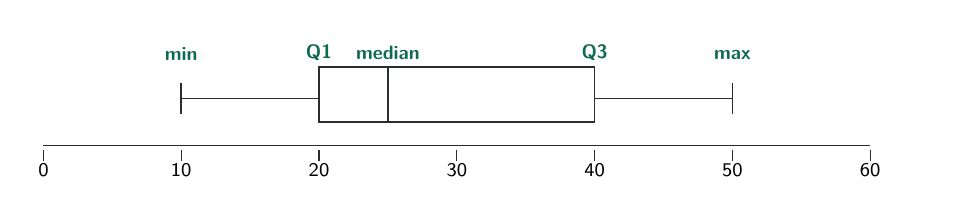
\begin{tikzpicture}[font=\sffamily\fontsize{7}{8}\selectfont]
\useasboundingbox (-2mm,-20mm) rectangle (112mm,0mm);
\draw[ink,line width=0.6pt] (17.50mm,-9mm) -- (35.00mm,-9mm);
\draw[ink,line width=0.6pt] (70.00mm,-9mm) -- (87.50mm,-9mm);
\draw[ink,line width=0.6pt] (17.50mm,-11mm) -- (17.50mm,-7mm);
\draw[ink,line width=0.6pt] (87.50mm,-11mm) -- (87.50mm,-7mm);
\draw[ink,fill=white,line width=0.6pt] (35.00mm,-12mm) rectangle (70.00mm,-5mm);
\draw[ink,line width=1pt] (43.75mm,-12mm) -- (43.75mm,-5mm);
\node[above,inner sep=0pt,text=accent] at (17.50mm,-4.2mm) {\bfseries min};
\node[above,inner sep=0pt,text=accent] at (35.00mm,-4.2mm) {\bfseries Q1};
\node[above,inner sep=0pt,text=accent] at (43.75mm,-4.2mm) {\bfseries median};
\node[above,inner sep=0pt,text=accent] at (70.00mm,-4.2mm) {\bfseries Q3};
\node[above,inner sep=0pt,text=accent] at (87.50mm,-4.2mm) {\bfseries max};
\draw[ink,line width=0.5pt] (0mm,-15mm) -- (105.00mm,-15mm);
\draw[ink,line width=0.4pt] (0.00mm,-15.5mm) -- (0.00mm,-16.9mm);
\node[below,inner sep=1pt] at (0.00mm,-16.8mm) {0};
\draw[ink,line width=0.4pt] (17.50mm,-15.5mm) -- (17.50mm,-16.9mm);
\node[below,inner sep=1pt] at (17.50mm,-16.8mm) {10};
\draw[ink,line width=0.4pt] (35.00mm,-15.5mm) -- (35.00mm,-16.9mm);
\node[below,inner sep=1pt] at (35.00mm,-16.8mm) {20};
\draw[ink,line width=0.4pt] (52.50mm,-15.5mm) -- (52.50mm,-16.9mm);
\node[below,inner sep=1pt] at (52.50mm,-16.8mm) {30};
\draw[ink,line width=0.4pt] (70.00mm,-15.5mm) -- (70.00mm,-16.9mm);
\node[below,inner sep=1pt] at (70.00mm,-16.8mm) {40};
\draw[ink,line width=0.4pt] (87.50mm,-15.5mm) -- (87.50mm,-16.9mm);
\node[below,inner sep=1pt] at (87.50mm,-16.8mm) {50};
\draw[ink,line width=0.4pt] (105.00mm,-15.5mm) -- (105.00mm,-16.9mm);
\node[below,inner sep=1pt] at (105.00mm,-16.8mm) {60};
\end{tikzpicture}
\end{textblock*}
\begin{textblock*}{158mm}(26mm,176.0mm)
{\fontsize{13}{16}\selectfont histogram: height $=$ frequency; median bar $=$ where the running total hits half}
\end{textblock*}
\begin{textblock*}{158mm}(26mm,182.5mm)
{\itshape\color{black!70}\fontsize{11}{14}\selectfont A long tail on the right: mode $<$ median $<$ mean. Symmetric: mean $=$ median.}
\end{textblock*}
% ---- Grouped data: least and greatest possible (y=196.6 h=38.6 end 235.2)
\cardbg{16}{196.6}{178}{38.6}
\pill{26}{199.6}{Grouped data: least and greatest possible}
\begin{textblock*}{158mm}(26mm,209.1mm)
{\fontsize{15}{18}\selectfont least mean: every value at the \textbf{bottom} of its class; greatest: at the \textbf{top}}
\end{textblock*}
\begin{textblock*}{158mm}(26mm,216.2mm)
{\fontsize{13}{16}\selectfont integer classes $0$--$9$ and $10$--$19$ (5 values each): least mean $5$, greatest $14$, difference $9$}
\end{textblock*}
\begin{textblock*}{158mm}(26mm,222.7mm)
{\itshape\color{black!70}\fontsize{11}{14}\selectfont For the median, find the two middle positions first (even count), then bound each. Midpoints give an estimate, not a bound.}
\end{textblock*}
\clearpage
\topicheader{7}{Data Analysis Edge Cases}
\pagekicker{Rules sheet -- 3/4}
\pagefooter{99}
\mbox{}%
% ---- Scatterplots and the line of best fit (y=33.0 h=45.5 end 78.5)
\cardbg{16}{33.0}{178}{45.5}
\pill{26}{36.0}{Scatterplots and the line of best fit}
\begin{textblock*}{158mm}(26mm,45.5mm)
{\fontsize{15}{18}\selectfont $y=mx+b$: \ slope $=$ change in $y$ per \textbf{one} unit of $x$}
\end{textblock*}
\begin{textblock*}{158mm}(26mm,52.6mm)
{\fontsize{13}{16}\selectfont $b=$ predicted $y$ at $x=0$ \qquad residual $=$ actual $-$ predicted}
\end{textblock*}
\begin{textblock*}{158mm}(26mm,59.1mm)
{\fontsize{13}{16}\selectfont $y=1.5x+8$, point $(12,30)$: \ residual $30-26=+4$ \quad ($+$ means above the line)}
\end{textblock*}
\begin{textblock*}{158mm}(26mm,65.7mm)
{\itshape\color{black!70}\fontsize{11}{14}\selectfont Inside the data range: prediction. Far outside it: extrapolation, unreliable. Check the intercept at $x=0$, not the left edge.}
\end{textblock*}
% ---- Reading a model from a graph (y=84.0 h=44.9 end 129.0)
\cardbg{16}{84.0}{178}{44.9}
\pill{26}{87.0}{Reading a model from a graph}
\begin{textblock*}{158mm}(26mm,96.5mm)
{\fontsize{15}{18}\selectfont slope from two far-apart points: $\dfrac{y_2-y_1}{x_2-x_1}$ \qquad point $(x_0,y_0)$: $b=y_0-mx_0$}
\end{textblock*}
\begin{textblock*}{158mm}(26mm,109.7mm)
{\fontsize{13}{16}\selectfont exponential $y=ab^x$: equal steps in $x$ multiply $y$ by $b$ \quad $4,\,6,\,9,\,13.5\Rightarrow b=1.5$, $a=4$}
\end{textblock*}
\begin{textblock*}{158mm}(26mm,116.1mm)
{\itshape\color{black!70}\fontsize{11}{14}\selectfont A far-away point tilts the line toward itself; removing it moves the slope and the intercept in opposite ways.}
\end{textblock*}
% ---- Two-way tables: conditional probability (y=134.5 h=50.5 end 185.0)
\cardbg{16}{134.5}{178}{50.5}
\pill{26}{137.5}{Two-way tables: conditional probability}
\begin{textblock*}{158mm}(26mm,147.0mm)
{\fontsize{15}{18}\selectfont $P(A\mid B)=\dfrac{\text{count}(A\text{ and }B)}{\text{count}(B)}$ \quad the ``given'' group is the denominator}
\end{textblock*}
\begin{textblock*}{158mm}(26mm,161.2mm)
{\fontsize{13}{16}\selectfont 40 like tea, 10 of them under 30: \ $P(\text{under }30\mid\text{tea})=\dfrac{10}{40}$ \qquad $P(\text{tea}\mid\text{under }30)\ne$ that}
\end{textblock*}
\begin{textblock*}{158mm}(26mm,172.1mm)
{\itshape\color{black!70}\fontsize{11}{14}\selectfont Reverse conditionals: with percents, build both parts (\,$0.55\cdot0.30$ and $0.45\cdot0.60$\,) and divide by the total of the group asked about.}
\end{textblock*}
% ---- Independence (y=190.5 h=39.3 end 229.8)
\cardbg{16}{190.5}{178}{39.3}
\pill{26}{193.5}{Independence}
\begin{textblock*}{158mm}(26mm,203.0mm)
{\fontsize{15}{18}\selectfont independent $\iff P(A\mid B)=P(A)\iff P(A\text{ and }B)=P(A)\,P(B)$}
\end{textblock*}
\begin{textblock*}{158mm}(26mm,210.3mm)
{\fontsize{13}{16}\selectfont in a table: the rate is the same in every row, e.g. $\dfrac{12}{40}=\dfrac{60}{200}=0.3$ \ $\Rightarrow$ independent}
\end{textblock*}
\begin{textblock*}{158mm}(26mm,221.2mm)
{\itshape\color{black!70}\fontsize{11}{14}\selectfont A parameter in the table: set the two rates equal and solve.}
\end{textblock*}
% ---- At least one; with and without replacement (y=235.3 h=46.3 end 281.6)
\cardbg{16}{235.3}{178}{46.3}
\pill{26}{238.3}{At least one; with and without replacement}
\begin{textblock*}{158mm}(26mm,247.8mm)
{\fontsize{15}{18}\selectfont $P(\text{at least one})=1-P(\text{none})$ \qquad independent: multiply}
\end{textblock*}
\begin{textblock*}{158mm}(26mm,255.1mm)
{\fontsize{13}{16}\selectfont $4$ items, each defective with probability $0.05$: \ $1-0.95^4$}
\end{textblock*}
\begin{textblock*}{158mm}(26mm,262.0mm)
{\fontsize{13}{16}\selectfont without replacement the pool shrinks: \ $5$ red, $3$ blue: $P(\text{both red})=\dfrac58\cdot\dfrac47$}
\end{textblock*}
\begin{textblock*}{158mm}(26mm,272.9mm)
{\itshape\color{black!70}\fontsize{11}{14}\selectfont Add the disjoint cases (e.g. both red, both blue). For ``least $n$ so that\,\ldots'' try values.}
\end{textblock*}
\clearpage
\topicheader{7}{Data Analysis Edge Cases}
\pagekicker{Rules sheet -- 4/4}
\pagefooter{100}
\mbox{}%
% ---- Expected counts and subgroup percents (y=33.0 h=38.0 end 71.0)
\cardbg{16}{33.0}{178}{38.0}
\pill{26}{36.0}{Expected counts and subgroup percents}
\begin{textblock*}{158mm}(26mm,45.5mm)
{\fontsize{15}{18}\selectfont expected count $=$ proportion $\times$ population}
\end{textblock*}
\begin{textblock*}{158mm}(26mm,52.6mm)
{\fontsize{13}{16}\selectfont 36 of 200 sampled $=18\%$; town of $5000$: \ $0.18\cdot5000=900$}
\end{textblock*}
\begin{textblock*}{158mm}(26mm,59.1mm)
{\itshape\color{black!70}\fontsize{11}{14}\selectfont Chain the proportions by multiplying. Percent of a subgroup: part $\div$ that subgroup's total, not the grand total.}
\end{textblock*}
% ---- Margin of error and intervals (y=76.5 h=39.0 end 115.6)
\cardbg{16}{76.5}{178}{39.0}
\pill{26}{79.5}{Margin of error and intervals}
\begin{textblock*}{158mm}(26mm,89.0mm)
{\fontsize{15}{18}\selectfont estimate $\pm$ margin of error $=$ \textbf{plausible} values for the population}
\end{textblock*}
\begin{textblock*}{158mm}(26mm,96.2mm)
{\fontsize{13}{16}\selectfont $62\%$ with margin of error $3$ points: \ plausible $59\%$ to $65\%$ (not exactly $62\%$)}
\end{textblock*}
\begin{textblock*}{158mm}(26mm,102.7mm)
{\itshape\color{black!70}\fontsize{11}{14}\selectfont 4 times the sample size halves the margin. Overlapping intervals: no difference shown. It is not a chance of error.}
\end{textblock*}
% ---- Study design: what can be concluded (y=121.1 h=57.6 end 178.6)
\cardbg{16}{121.1}{178}{57.6}
\pill{26}{124.1}{Study design: what can be concluded}
\begin{textblock*}{158mm}(26mm,133.6mm)
{\fontsize{10.5}{13}\selectfont\renewcommand{\arraystretch}{1.25}
\begin{tabular}{|p{66mm}|p{74mm}|}\hline
\cellcolor{accent}\textcolor{white}{\bfseries Study design} & \cellcolor{accent}\textcolor{white}{\bfseries Conclusion allowed}\\ \hline
random sample \textbf{and} random assignment & cause for the whole population\\ \hline
random sample, no random assignment & association for the population (no cause)\\ \hline
random assignment of volunteers & cause, for people like the volunteers\\ \hline
neither (self-selected, convenience) & association in the sample; biased\\ \hline
\end{tabular}}
\end{textblock*}
\begin{textblock*}{158mm}(26mm,165.8mm)
{\itshape\color{black!70}\fontsize{11}{14}\selectfont Generalize only to the population the sample was drawn from. A flawed sampling method cannot be fixed by a larger sample.}
\end{textblock*}
% ---- New words (y=184.1 h=68.5)
\cardbg{16}{184.1}{178}{68.5}
\pillw{26}{187.1}{NEW WORDS ~\textperiodcentered~ YANGI SO'ZLAR}
\begin{textblock*}{80mm}(26mm,196.6mm)
{\fontsize{10.5}{12}\selectfont
\begin{tabular}{@{}>{\bfseries}p{37mm}p{36mm}@{}}
\cellcolor{accent}\textcolor{white}{\sffamily English} & \cellcolor{accent}\textcolor{white}{\sffamily O'zbekcha}\\
\rowcolor{badge!45} mean & {\itshape o'rtacha qiymat}\\
\rowcolor{white} median & {\itshape mediana}\\
\rowcolor{badge!45} mode & {\itshape moda}\\
\rowcolor{white} range & {\itshape variatsiya oralig'i}\\
\rowcolor{badge!45} standard deviation & {\itshape standart og'ish}\\
\rowcolor{white} outlier & {\itshape chetga chiqqan qiymat}\\
\rowcolor{badge!45} quartile & {\itshape kvartil}\\
\end{tabular}}
\end{textblock*}
\begin{textblock*}{80mm}(108mm,196.6mm)
{\fontsize{10.5}{12}\selectfont
\begin{tabular}{@{}>{\bfseries}p{37mm}p{36mm}@{}}
\cellcolor{accent}\textcolor{white}{\sffamily English} & \cellcolor{accent}\textcolor{white}{\sffamily O'zbekcha}\\
\rowcolor{badge!45} line of best fit & {\itshape eng mos to'g'ri chiziq}\\
\rowcolor{white} residual & {\itshape qoldiq (chetlanish)}\\
\rowcolor{badge!45} conditional probability & {\itshape shartli ehtimollik}\\
\rowcolor{white} independent events & {\itshape erkli hodisalar}\\
\rowcolor{badge!45} sample / population & {\itshape tanlanma / bosh to'plam}\\
\rowcolor{white} margin of error & {\itshape xatolik chegarasi}\\
\rowcolor{badge!45} bias & {\itshape tarafkashlik}\\
\end{tabular}}
\end{textblock*}
\end{document}
